\chapter{Symbolic Derivation}

We give a detailled description of how automatic differentiation is handled in {\tt MMVII}.
This description is for curious readers or possibly programmer who will have to maintain this part.
For devlopper that will only use these  automatic differentiation facilities, probably the 
short introduction given in~\ref{Compute:Deriv:SysNL} is sufficient.

%-----------------------------------------------------
%-----------------------------------------------------
%-----------------------------------------------------

\section{introduction}


%-----------------------------------------------------
\subsection{Motivations}

The computation of derivatives of a given function are central point in metrology
where it is used in Gauss-Newton-like iteration.  There is basically $4$ methods
for computing derivative :

\begin{itemize}
    \item  computing "by hand", i.e a human apply the rules of derivation as
           learned at school;  this method is perfectly manageable with "small"
           function, but with "complicated" function as colinearity equation with many distorsion parametersr,
           it is error prone, difficult to maintain, and potentially not so fast as there
           are simplification that human may miss;

    \item  numericall derivative, for example with a $2$ variable function use equation as~\ref{NumDer}
           where $\epsilon_x$ is a "small" value relative to variable $x$;
           this method as the advantage of simplicity, if you know the function you know the derivative;
           it has $2$ drawbacks :  first issue, it's not always easy to define a good small value,  too small
           creates numericall problem, not enough is unacurate, and with heterogeneous variable the small
            value must be defined for each variable;  second issue, it is relatively slow, with $N$  variable
           we must have $2N$ evaluation of $F$;

     \item jet method as used in CERES, see~\cite{CERES} for detailled description, it's not error
           prone as "hand crafted", there is no problem of accuracy, they are faster than 
           numerical derivatives; however they are relatively slow compared to formal methods;

     \item formal method, that "more or less" do the same thing than "human computation" but do
           it automatically; they are separated between automatic differenciation that anlyse the code
           and symbolic differenciation that construct a tree representation, but to our mind this separation
           is a bit artificial and their performance are similar;  {\tt MMVII} uses symbolic differenciation;
           the use is a bit more complicated than jet but can be significatively faster  than jet on complicated
           formulas.
\end{itemize}

\begin{equation}
    \frac{\partial F(x_0,y_0)}{\partial x} \approx \frac{F(x_0 + \epsilon_x,y_0) - F(x_0-\epsilon_x,y_0)}{2* \epsilon_x}
     \label{NumDer}
\end{equation}

%-----------------------------------------------------
\subsection{Code localization}

The code on automatic differenciation has been organized in such a way that 
the code can be reused outside the {\tt MMVII} library. It's a header only code
that is located in {\tt MMVII/include/SymbDer/}.


The code that use it more specifically for task adressed in  {\tt MMVII},
as photogrammetry or compensation in general, are to be found in the
folder  {\tt MMVII/src/SymbDerGen}.


%-----------------------------------------------------
\subsection{Tree/DAG representation}

\begin{figure}
\centering
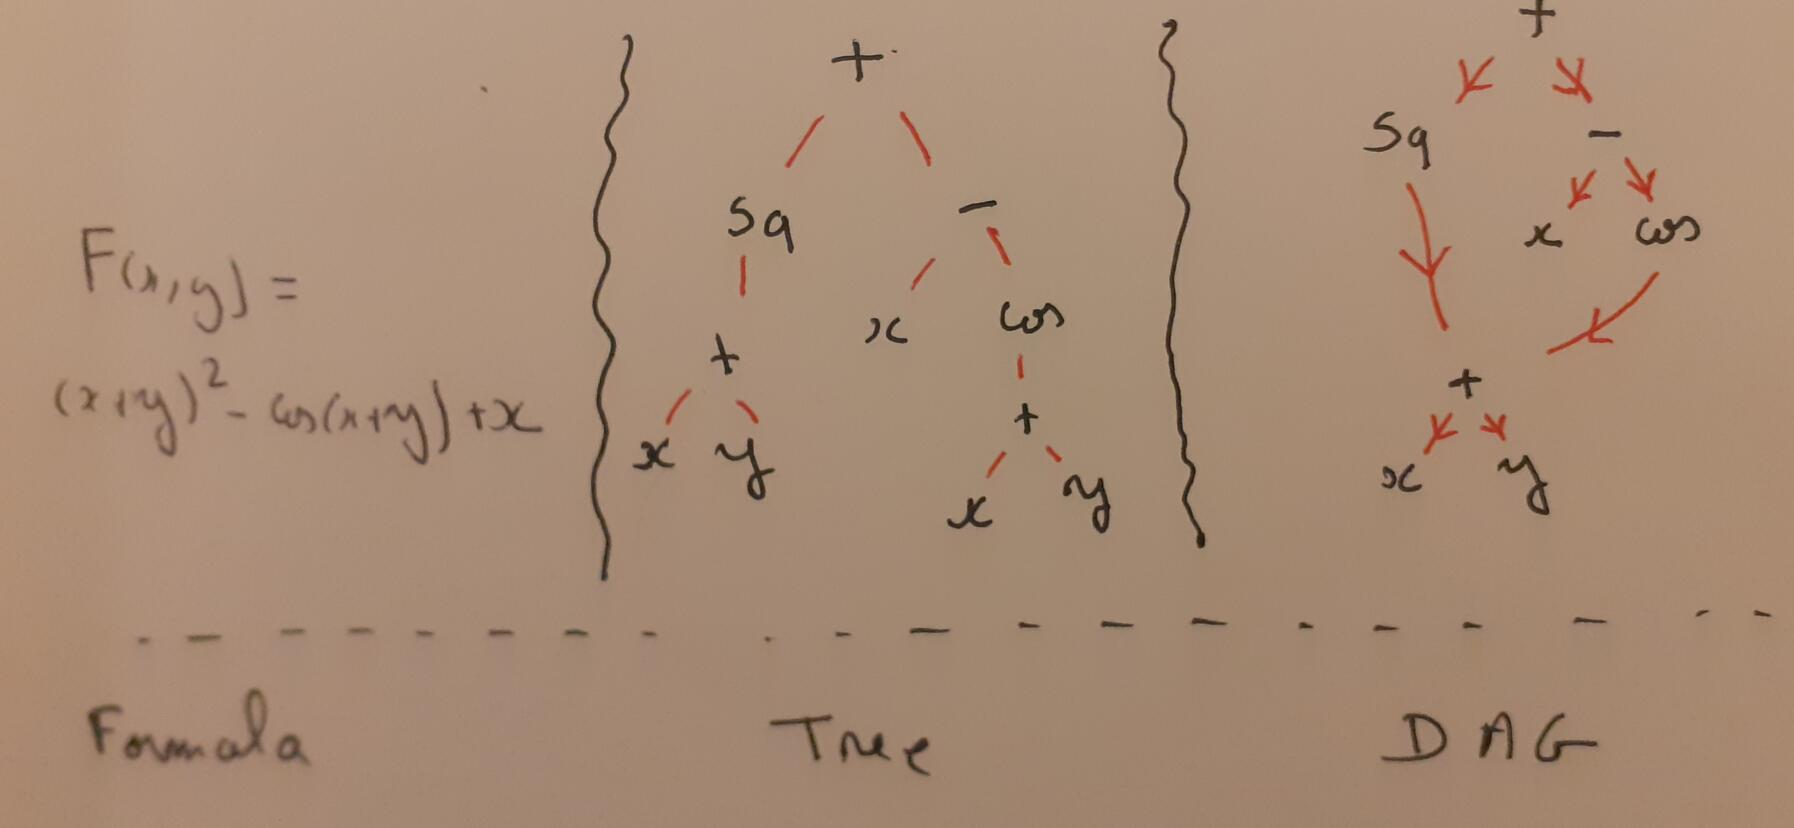
\includegraphics[width=12cm]{Programmer/ImagesProg/Tree.jpg}
\caption{Representation of formulas}
\label{fig:TreeFormula}
\end{figure}

The classic aproach is to represent the mathematicall formulas as tree (or more precizely as we will see "DAG"=  directly acyclic graph).
These trees can be described recursively :

\begin{itemize}
   \item  constant ($0,1,\pi \dots$)  and fonction corresponding to variables ($x_1,x_2,\dots ,x_{144} \dots$)
          are  atomic formulas, their tree has one node labeled by the contant or the variable;

   \item if $Op$ is a unary operator, like $cos, sin, exp $ for example,  and $F$ is a formula then $Op(F)$ is a 
         formula, its trees is a node labeled by $Op$ and has one son corresponding to the tree of $F$;

   \item if $Op$ is a binary operator, like $+,* $ for example,  and $F_1$  and $F_2$ are  formulas then $Op(F_1,F_2)$ is a 
         formula,  its trees is a node labeled by $Op$ and has two son corresponding to the trees of $F_1$ and $F_2$.
\end{itemize}


Figure~\ref{fig:TreeFormula} represent the tree for the formula $F(x,y) = (x+y)^2 +x - \cos(x+y)$. 
In the formula, we see that the sub-formula $x+y$ appears twice in the $F$, to optimize the computation,
a directed acyclic graph (DAG) is prefered to tree;  a DAG  is still a hierarchy, but the difference
if that a node can have several parents, which avoid duplication as the same formula can be shared.
The right part of figure~\ref{fig:TreeFormula} correspond to DAG for formula $F$.


The difference in efficiency between a tree and a DAG can be very significant 
in complicated multiple formula  (maybe up to $10$). By multiple formula we mean formula that return several values;
in differenciation we will compute $F$ but also all its derivatives and it often happen that
the same sub-formula appears in several partial derivatives.  In our example we
have $\frac{\partial F}{\partial x} = 2*(x+y) -1 + \sin(x+y)$ and $\frac{\partial F}{\partial y} = 2*(x+y) + \sin(x+y)$ ,
and figure~\ref{fig:DagMultiformula} represents the DAG for the multiple formula
$F,\frac{\partial F}{\partial x},\frac{\partial F}{\partial y}$.



\begin{figure}
\centering
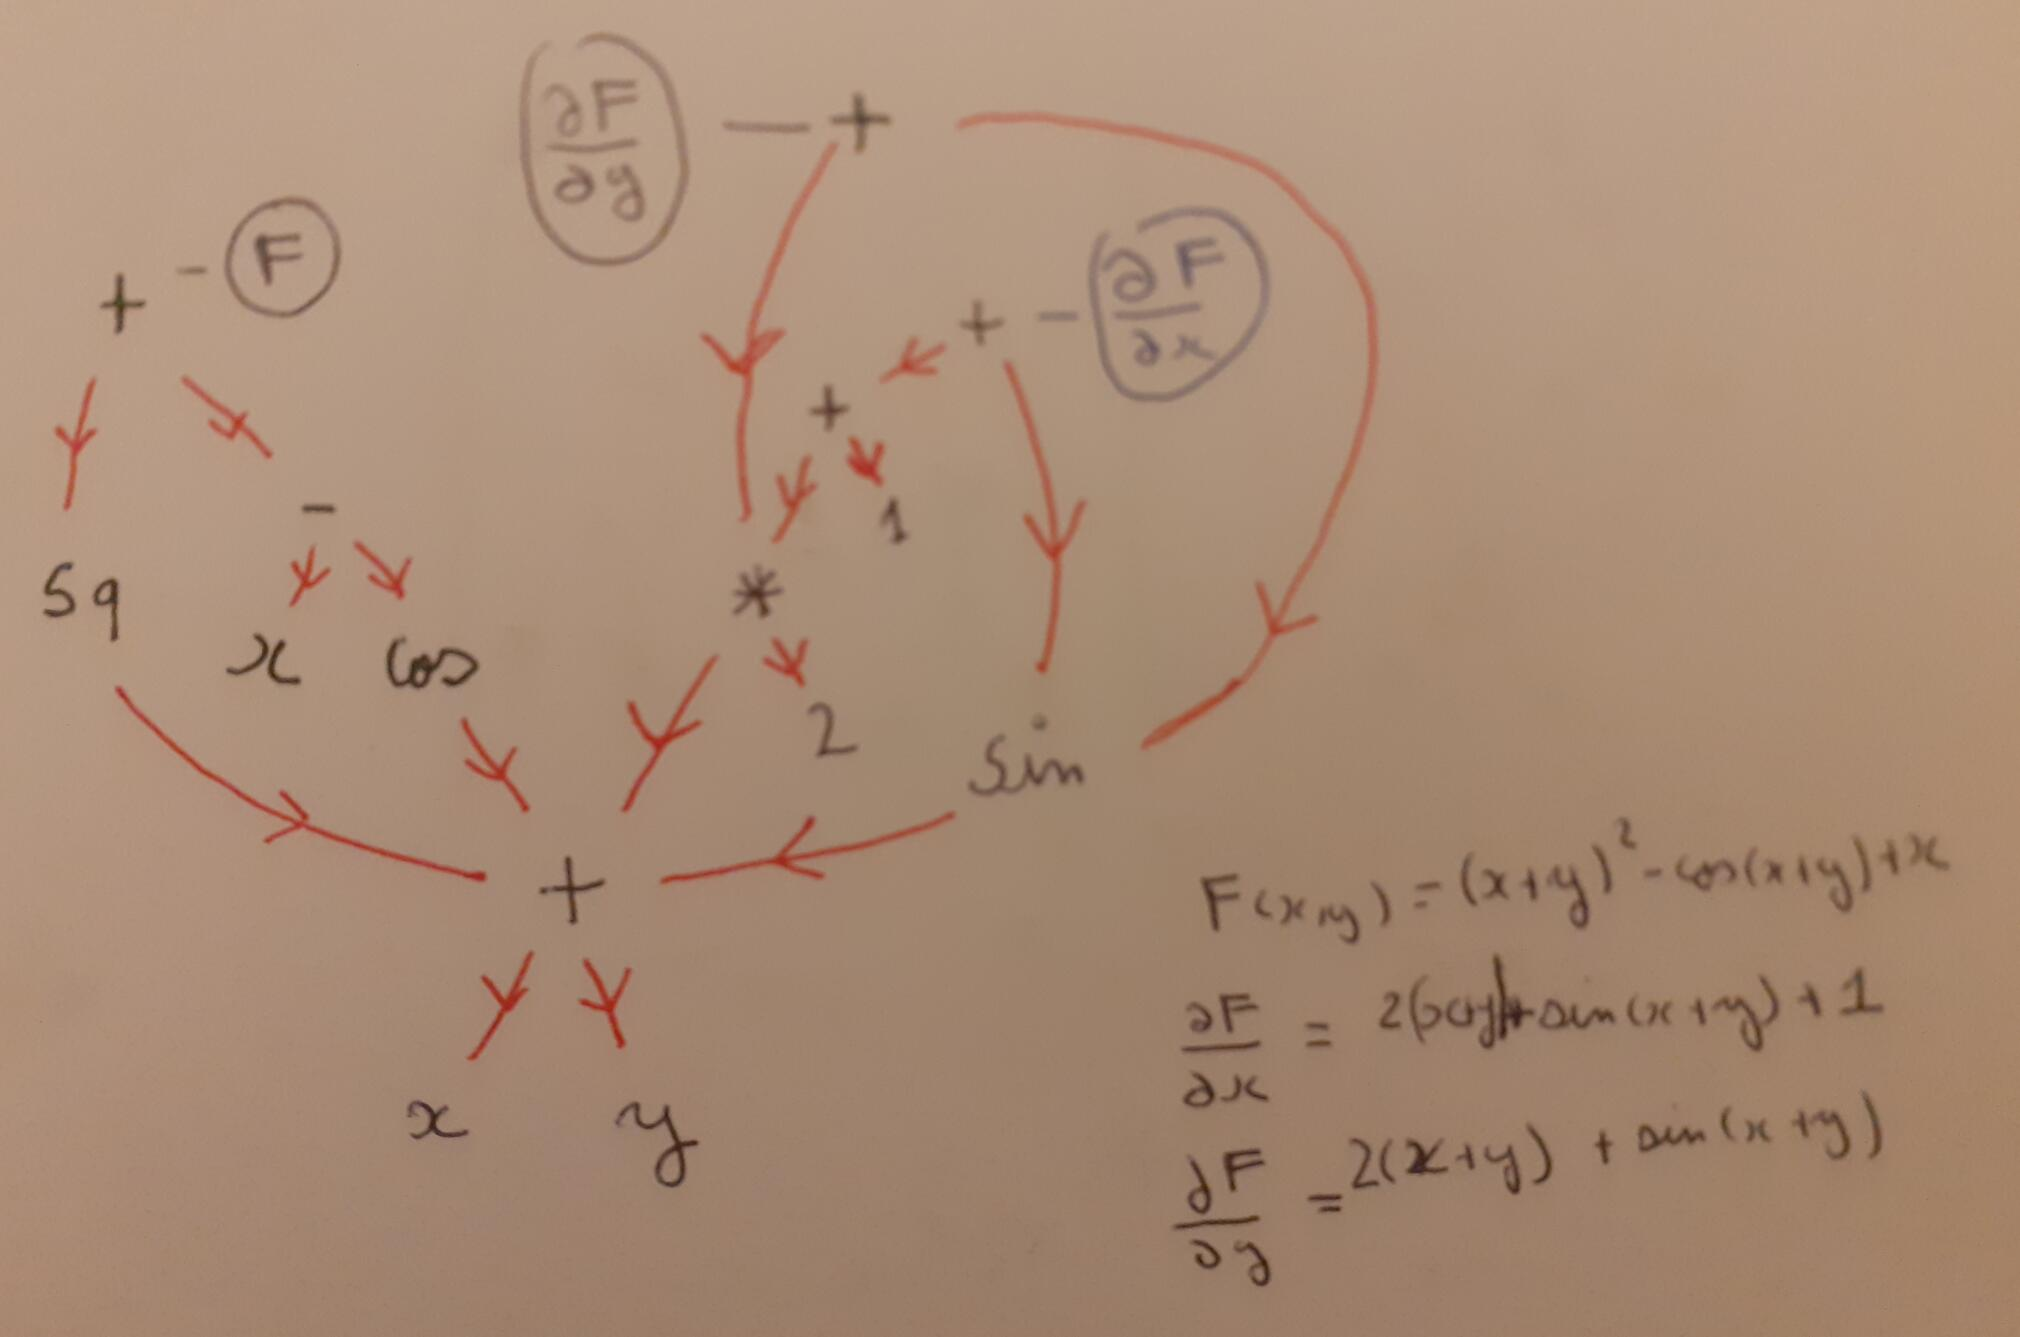
\includegraphics[width=12cm]{Programmer/ImagesProg/DAG.jpg}
\caption{DAG for a multiple formula  $[F,\frac{\partial F}{\partial x}, \frac{\partial F}{\partial y}]$ with $F(x,y) = (x+y)^2 +x - \cos(x+y)$}
\label{fig:DagMultiformula}
\end{figure}


%-----------------------------------------------------
%-----------------------------------------------------
%-----------------------------------------------------

\section{Code usable outside  MMVII}

\subsection{general organization}

The code is located in  {\tt MMVII/include/SymbDer/}.

The key-file is {\tt SymbolicDerivatives.h}  where is defined   the key-classes   {\tt cFormula/cImplemF},
cFormula being simply pointer on cImplemF,  ({\tt cImplemF} is the real class containing the date, while
{\tt cFormula} are the classes manipulated externally as we want permanent objet  semantic).


A formula is the {\tt C++} equivalent of the tree/DAG, the specification of the formula :

\begin{itemize}
	\item  a formula contain a set of sub-formula (currently between $0$ en $2$);
\end{itemize}







\subsection{DAG construction}
